\documentclass{article}

\usepackage{amsmath}
\usepackage{amssymb}

\usepackage{tikz}
\usetikzlibrary{positioning}

\tikzstyle{block} = [draw, rectangle, align=center]
\tikzstyle{op} = [draw, inner sep=1pt, circle]

\newcommand{\real}{\mathbb{R}}

\title{Physiological Signal Classification with Recursive Sequence Reduction}
\author{Daniel Schulman}

\begin{document}
\maketitle

\section{Introduction}

Classification of physiological signals, such as electromyography (EMG), electroencephalography (EEG), and electrocardiography (ECG), is a common task in applications of artificial intelligence and machine learning to healthcare.
In the last few years, deep learning models have become state-of-the-art in many physiological signal classification tasks, in several cases achieving performance superior to human experts.

Physiological signals differ from many of the domains that deep learning models were originally developed on, such as computer vision.
They typically have fairly high temporal resolution, so that even brief recordings of signals have many more samples than other types of sequential data (e.g. natural language).
Signal length often varies, and models that are designed around data with fixed dimensionality (e.g. CNNs) can be awkward.

In this paper, we introduce a novel approach --- a \emph{recursive sequence reduction network} (RSRNs) --- that provides a simple baseline approach that is well-suited to physiological signal classification tasks.
RSRNs handle long sequences and varying-length sequence, and can deliver competitive performance with relatively small models, which may make usage feasible on edge devices with limited memory or computational power.

We first introduce RSRNs, then present experiments demonstrating performance on a set of benchmark tasks.
We compare and contrast RSRNs to other models, and we discuss applications where RSRNs may be suitable.

\section{Recursive Sequence Reduction Networks}

One way we can understand a sequence classification task is as learning a transformation from a variable-dimension input (a sequence) to a fixed-dimension output (e.g. a vector of class probabilities).
We consider a function $f(x,\theta)$ that operates on sequences with a fixed number of features ($M$) but arbitrary length.
If $x \in \real^{M \times N}$, then $f(x, \theta) \in \real^{M \times N'}$, where $1 \leq N' \leq N/K$ for some $K \in \mathbb{Z}$, $K \geq 2$.
That is, $f$ reduces a sequence of arbitrary length ($N$) to a sequence that is a fraction of the length.
We can apply $f$ recursively to reduce a sequence to a fixed-dimension feature vector.

\begin{equation}
    F(x, \theta) =
    \begin{cases}
        x &\text{if } x \in \real^{M \times 1} \\
        F(f(x, \theta), \theta) &\text{otherwise}
    \end{cases}
\end{equation}

In our RSRNs, we model $f$ with a convolutional network; specifically, a variant of a resnet, using strided convolutions to reduce sequence length at each step.
However, in typical usage of a resnet-style network, we would stack multiple layers to create a deep network.
Here, we simply apply the \emph{same} layers (i.e. sharing weights) repeatedly until the sequence is reduced.

\begin{figure}
\centering
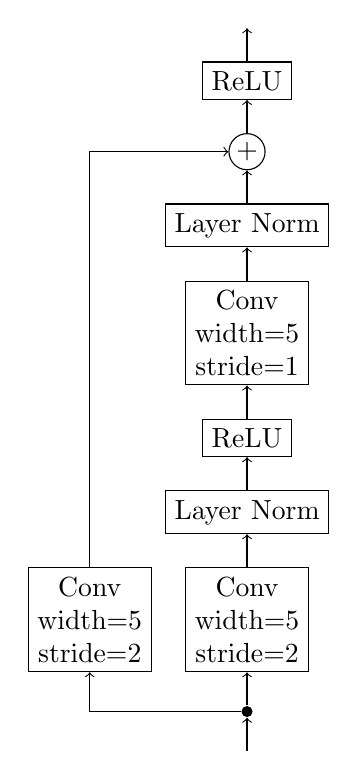
\begin{tikzpicture}[node distance=12pt]
\node (input) [coordinate] {};
\node (split) [fill, circle, inner sep=0pt, minimum size=4pt, above=of input] {};
\draw [->] (input) -- (split);
\node (conv1r) [block, above=of split] {Conv\\width=5\\stride=2};
\draw [->] (split) -- (conv1r);
\node (conv1l) [block, left=of conv1r] {Conv\\width=5\\stride=2};
\draw [->] (split) -| (conv1l);
\node (ln1) [block, above=of conv1r] {Layer Norm};
\draw [->] (conv1r) -- (ln1);
\node (relu1) [block, above=of ln1] {ReLU};
\draw [->] (ln1) -- (relu1);
\node (conv2) [block, above=of relu1] {Conv\\width=5\\stride=1};
\draw [->] (relu1) -- (conv2);
\node (ln2) [block, above=of conv2] {Layer Norm};
\draw [->] (conv2) -- (ln2);
\node (sum) [op, above=of ln2] {$+$};
\draw [->] (conv1l) |- (sum);
\draw [->] (ln2) -- (sum);
\node (relu2) [block, above=of sum] {ReLU};
\draw [->] (sum) -- (relu2);
\node (output) [coordinate, above=of relu2] {};
\draw [->] (relu2) -- (output);
\end{tikzpicture}
\caption{A Basic Block}
\end{figure}

\end{document}